% ----------------------------------------------------------
% Subseção Expansão lógica
% ----------------------------------------------------------
\subsection{Expansão lógica}
A lógica primordial (negação de si) cria expansões lógicas infinitas. Uma expansão lógica é análoga a um universo. O primeiro momento lógico é o início de uma dessas expansões, porém existem infinitas possibilidades de negação do primeiro momento lógico, o que revela infinitas expansões lógicas.
	\begin{figure}[H]
	\caption{Momentos lógicos iniciais}
	\label{fig:third_logical_moment}
	\centering
	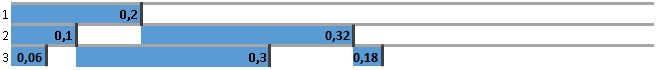
\includegraphics[scale=.85]{sections/images/third_logical_moment.jpg}
	\floatfoot{Exemplo dos três primeiros momentos de uma expansão.}%\footnotemark}
	\end{figure}
	%\footnotetext{Fonte: note}

Com base na Figura \ref{fig:third_logical_moment} pode-se extrair as seguintes observações em relação ao primeiro, segundo e terceiro momentos lógicos:
	\begin{description}
	   \item[Primeiro momento lógico] A negação da lógica primordial a si, a subdivide em duas unidades, duas sub-lógicas. Apesar dessas partes terem proporções diferentes, elas exprimem as mesmas quantidades de pontos ou possibilidades de mudança, uma vez que são representações da lógica primordial, que \textit{ad infinitum}. A parte fracionada em azul representa a proporção da negação lógica em relação à sua unidade.
	   \item[Segundo momento lógico] É gerado pela negação das duas sub-lógicas primordiais fracionadas no primeiro momento lógico, ou seja, o segundo momento lógico é uma negação do primeiro. Na impossibilidade dessas sub-lógicas continuarem negando a si, por qualquer instante que seja, faria com que elas fossem incapazes de negar suas duas unidades do todo e por consequência o faria \underline{SER}. As partes fracionadas em azul representam a proporção da negação lógica em relação às suas respectivas unidades.
	   \item[Terceiro momento lógico] Decorre da negação do segundo momento lógico, assim como o segundo momento lógico decorre da negação do primeiro e assim por diante.
	\end{description}

A cada negação ou subnegação da lógica primordial, seus novos valores são influenciados pelos valores adjacentes do momento lógico anterior. Na figura \ref{fig:imposition_of_binomial_expansion}, a lógica primordial nega a si gerando o primeiro momento lógico com o valor [0,2].  No segundo momento lógico, suas subdivisões estão contidas no limite imposto pelo valor do primeiro momento lógico. Os pontos do terceiro momento lógico, por exemplo, sofrem as imposições dos valores do segundo momento lógico que por sua vez sofrem a imposição do primeiro. O triângulo de pascal tem propriedades interessantes sobre essa relação. 
	\begin{figure}[H]
	\caption{Imposição da expansão lógica}
	\label{fig:imposition_of_binomial_expansion}
	\centering
	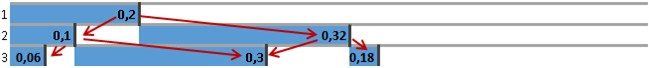
\includegraphics[scale=.85]{sections/images/imposition_of_binomial_expansion.jpg}
	\floatfoot{Imposição acumulativa aos momentos lógicos descendentes.}%\footnotemark}
	\end{figure}
	%\footnotetext{Fonte: note}

No triângulo de pascal, Figura \ref{fig:pascal_triangle}, cada número é os dois números acima mais próximos somados. Esse número representa quantos diferentes possíveis caminhos levam até ele. Por exemplo, o número [4], na Figura \ref{fig:pascal_triangle}, representa os quatro diferentes caminhos que levam até ele. Os coeficientes binômias encontrados no triangulo de Pascal representam apenas as quantidades de imposições sofridas por cada valor de um momento lógico. Um outro aspecto interessante do triângulo de pascal é a sequência de Fibonacci, Figura \ref{fig:pascal_triangle_fibonacci} \cite{mathisfun_pascal_triangle}.  
\enlargethispage{\baselineskip}
	\begin{figure}[H]
	\centering
		\begin{subfigure}[H]{0.47\linewidth}
		\centering
		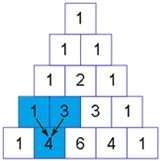
\includegraphics[width=.55\linewidth]{sections/images/pascal_triangle.jpg}
		\caption{}
		\label{fig:pascal_triangle}
		\end{subfigure}
	\hfill
		\begin{subfigure}[H]{0.47\linewidth}
		\centering
		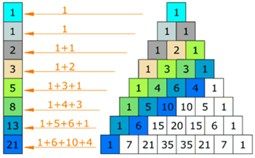
\includegraphics[width=.9\linewidth]{sections/images/pascal_triangle_fibonacci.jpg}
		\caption{}
		\label{fig:pascal_triangle_fibonacci}
		\end{subfigure}%
	\caption{Características do triângulo de Pascal}
	\floatfoot{Fonte: MathsIsFun, 2019. \protect\footnotemark}
	\end{figure}
	\footnotetext{\url{www.mathsisfun.com/pascals-triangle.html}}
